\documentclass[12pt]{article}
\usepackage{hyperref}
\usepackage{graphicx}
\usepackage{mathtools}
\usepackage[margin=1in, paperwidth=8.5in, paperheight=11in]{geometry}
\begin{document}
\title{Istanbul Technical University- Spring 2017 \\ BLG527E Machine Learning \\ Homework 4}
\author{Omid Abdollahi Aghdam \\
student number: 504151520\\
\href{mailto:abdollahi15@itu.edu.tr}{abdollahi15@itu.edu.tr}\\
\href{mailto:abdollahi.omid@gmail.com}{abdollahi.omid@gmail.com}
}
\date{\today}
\maketitle
\newpage
\textbf{Q1)} This is a Head-to-Head connection and we use diagnostic inference (\ref{diaginf}) to compute the probability. We use the given marginal and conditional probabilities to find $P(G=0 | F=1)$ and $P(G=0)$ and the replace them in the \ref{diaginf}.\\

\begin{equation}\label{diaginf}
	P(F=1 | G =0) = \frac{P(G=0 | F=1)P(F=1)}{P(G=0)}
\end{equation}

We calculate $P(G=0)$ by marginalizing over the joint probabilities.

\begin{equation}\label{joint}
	\begin{aligned}
		P(G=0) &= \Sigma_{B,F} P(G,B,F)\\
		&= P(G=0 | B=1, F=1)P(B=1|F=1) + P(G=0 | B=0, F=0)P(B=0|F=0)\\
		&+ P(G=0 | B=1, F=0)P(B=1|F=0) + P(G=0 | B=0, F=1)P(B=0|F=1) \\
		&= 0.315
	\end{aligned}
\end{equation}

To compute $P(G=0 | F=1)$, which is a causal (predictive) inference, we marginalize over B.

\begin{equation}\label{causal}
	\begin{aligned}
		P(G=0 | F=1) &= \Sigma_{B} P(G,B,F)\\
		&= P(G=0 | B=1, F=1)P(B=1|F=1) + P(G=0 | B=0, F=1)P(B=0|F=1)\\
		&= P(G=0 | B=1, F=1)P(B=1) + P(G=0 | B=0, F=1)P(B=0)\\
		&= 0.26
	\end{aligned}
\end{equation}
We replace the result of \ref{causal} and \ref{joint} in \ref{diaginf} to compute $P(F=1 | G =0)$.
\begin{equation}
	\begin{aligned}
		P(F=1 | G =0) &= \frac{0.26 \times 0.9}{0.315}\\
		&= 0.743
	\end{aligned}
\end{equation}
\textbf{Q2)} Observation sequence is $\{O_1 = Red, O_2=Red\}$, we calculate $P(O | A, B, \pi)$ using forward variable.\\

\textbf{Initialization:}\\
We denote state 1 and 2 with $S_1, S_2$ respectively.
\begin{equation}
	\begin{aligned}
		\alpha_{t=1}(S_1) &= \pi_{S_1}b_{S_1}(Red)\\
						&= 0.2 \times 0.3\\
						&=0.06
	\end{aligned}
\end{equation}

\begin{equation}
	\begin{aligned}
		\alpha_{t=1}(S_2) &= \pi_{S_2}b_{S_2}(Red)\\
		&= 0.8 \times 0.5\\
		&=0.4
	\end{aligned}
\end{equation}

\textbf{Recursion:}\\
\begin{equation}
	\begin{aligned}
		\alpha_{t=2}(S_1) &= [ \Sigma_{i=1}^2 \alpha_{t=1}(i)a_{i1}]b_{S_1}(Red)\\
		&= [0.06 \times 0.6 + 0.4 \times 0.5]0.3\\
		&= 0.0708
	\end{aligned}
\end{equation}

\begin{equation}
	\begin{aligned}
		\alpha_{t=2}(S_2) &= [ \Sigma_{i=1}^2 \alpha_{t=1}(i)a_{i2}]b_{S_2}(Red)\\
		&= [0.06 \times 0.4 + 0.4 \times 0.5]0.5\\
		&= 0.112
	\end{aligned}
\end{equation}

\begin{equation}
	\begin{aligned}
		p(O | A, B, \pi) &= \Sigma_{i=1}^2 \alpha_T(i)\\
		&=\alpha_{t=2}(S_1) + \alpha_{t=2}(S_2)\\
		&= 0.0708 + 0.112\\
		&= 0.1828
	\end{aligned}
\end{equation}

\textbf{Q3a)} We have selected Keras. It is written with python and has Tensorflow or Theano as backend and provides high level API for implementing deep learning models. Using keras we can implement any artificial neural network architecture in a short amount of time.\\

\textbf{Q3b)} We implement a three layer neural network model using keras (lines 94-101 in file hw4.py). Afterwards, we tune the hyper-parameters  (lines 103-127) and train the best model on whole train data. Train, test time, and confusion matrices will be outputted on terminal by running hw4.py. Figures \ref{fig:train}, \ref{fig:test}, shows the train and test confusion matrices respectively.\\

\begin{figure}[h] 
	\begin{center}
		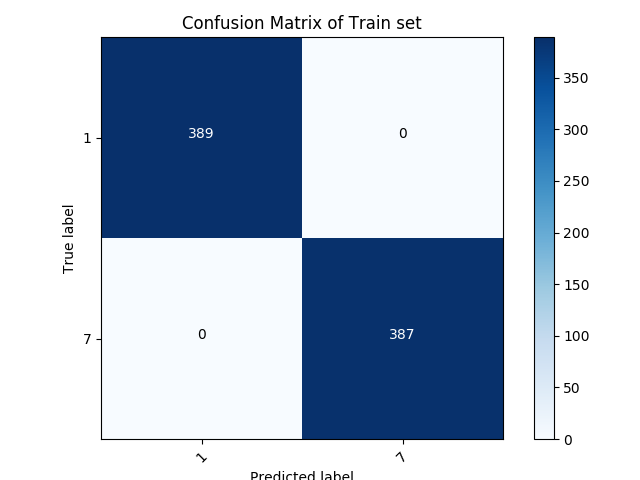
\includegraphics[width=3in]{train.png}
		\caption{Confusion Matrix of Train set.}
		\label{fig:train}
	\end{center}
\end{figure}  
\begin{figure}[h] 
	\begin{center}
		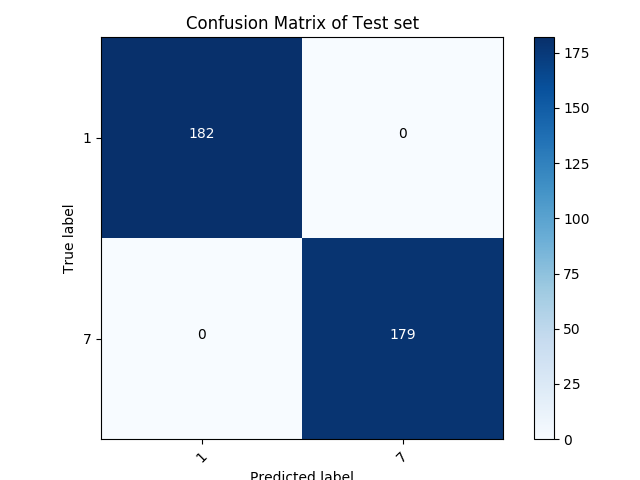
\includegraphics[width=3in]{test.png}
		\caption{Confusion Matrix of Train set.}
		\label{fig:test}
	\end{center}
\end{figure}  

\end{document}